\begin{solution}
The answer is $\pi + 1$.\\[0.2cm]

We first prove that if the cat's speed is less than $\pi + 1$ times the mouse's speed, there is a strategy for the mouse to escape the circle. Recall that the length of the circle is 1m. Now, consider the imaginary red circle whose center is the same as the center of the problem's circle but it's radius is $1/(1+\pi)$m.
\begin{center}
	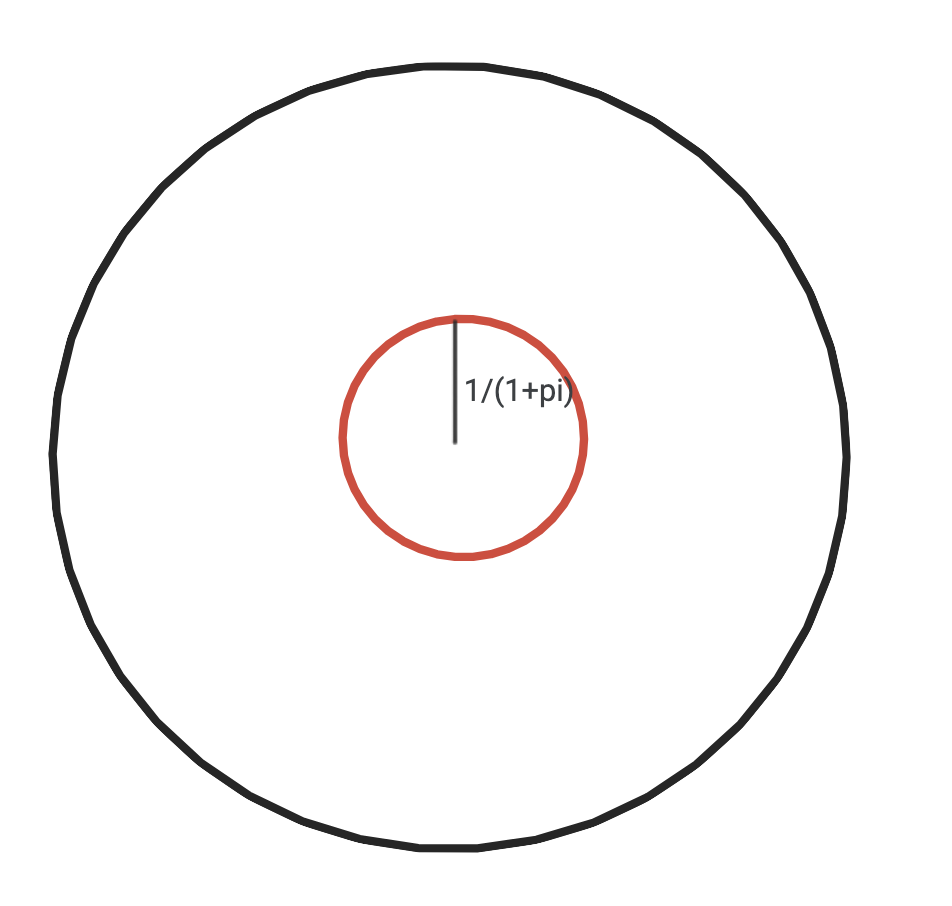
\includegraphics{68/figs/68_sol1.png}
\end{center}
In this case, the mouse can escape the black circle with the following strategy:
\begin{enumerate}
	\item The mouse first moves towards an arbitrary point of the red circle without caring about the cat's movement.
	\item When the mouse reaches a point of the red circle, it only moves on the border of the red circle. Let's define the projection of the cat's place on the red circle as the intersection of the red circle with the segment between cat's position and the center of the circles. If we extend this segment from both ends, it intersects the red circle on one more point which is the opposite of the first intersection. We call the second point, \textit{the opposite projection of cat's place} on the red circle.\\
	\begin{center}
		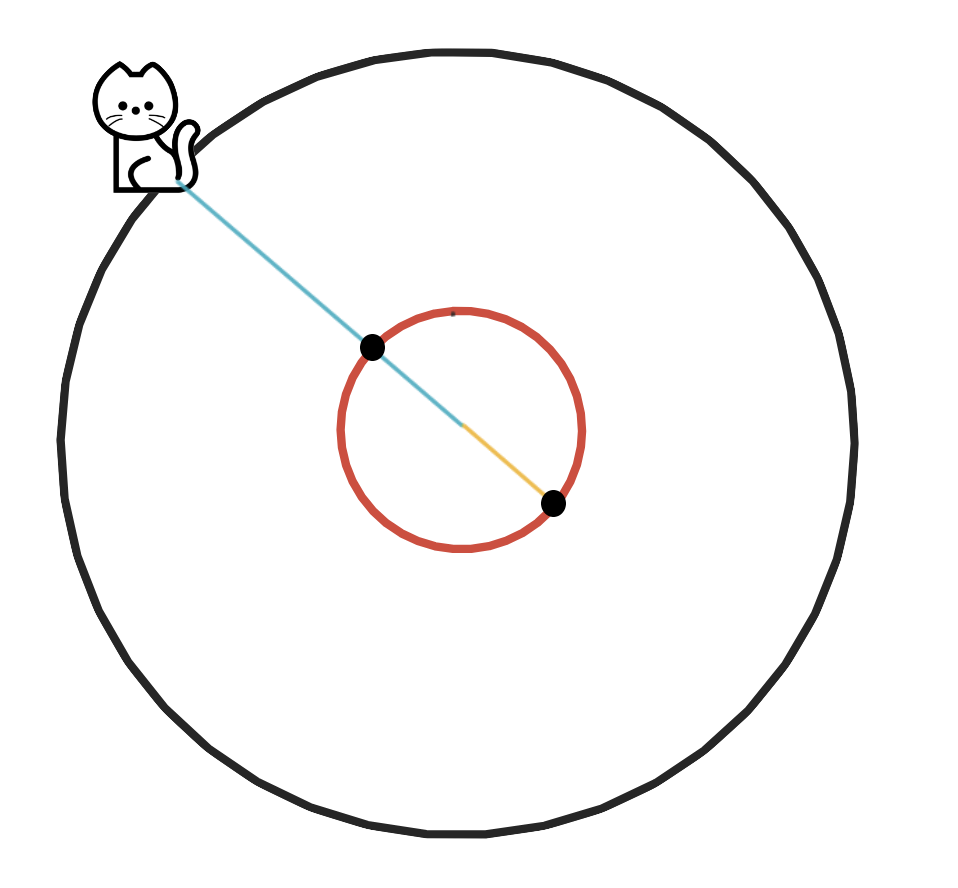
\includegraphics{68/figs/68_sol2.png}
	\end{center}
	In this step, the mouse always moves towards the opposite projection of the cat's place on the red circle. Notice that since the cat moves on a circle whose radius is $1+\pi$ times that of the red circle but it's speed is less than $1+\pi$ times the speed of the mouse, the mouse can eventually reach the opposite projection of the cat's place on the red circle.
	\item As soon as the mouse reaches the opposite projection of the cat's place on the red circle, it directly goes towards the closest point of the black circle. Notice that since the radius of the red circle is $1/(1+\pi)$ and the radius of the black circle is $1$, then the distance that the mouse has to travel is $1-1/(1+\pi) = \pi / (\pi+1)$. In order for the cat to catch the mouse, it has to travel a distance of $\pi$. However, since the cat's speed is less that $1+\pi$ times that of the mouse, the mouse can reach that point earlier than the cat and thus escape the circle.
\end{enumerate}


The next part is to show that if the cat's speed is at least $1+\pi$ times the speed of the mouse, it can always catch the mouse. The cat's strategy in this case it easy. It does not move at all whenever the mouse is moving inside the red circle. As soon as the mouse comes outside the red circle, the cat always moves towards the point on the black circle which is closest to the mouse. Since the cat's speed is at least $1+\pi$ times that of the mouse, and at any time the distance that the cat has to move is at most $1+\pi$ times the distance that the mouse has to travel in order to escape the circle, the cat can always catch the mouse if it crosses the circle.
\end{solution}
